% ==========================================
% Thesis Report - Testing ( waltj3 )
% ==========================================
\chapter{Testing}

\section{Framework Tests}
\label{sec:crfTesting}

\subsection{Early Tests}
\label{sec:EarlyTests}\hfill\\
Because of the fact that the real CAVE setup had to be configured first, we did the early tests on our local machines on Window and Linux with different Equalizer configurations. Some of these configurations simulated something like a multipipe environment and looked at least technically pretty similar to tests in the real CAVE. Later in the project we managed to setup our CAVE clone rendering client with four GPUs and LCD monitors. This was the time when we first realised that our framework did not work with a lot of early test applications on this multipipe machine. After some debugging and sleepless nights the errors could be tracked down as memory abuse. This happened because we first used a lot of the original \gls{osg} demo applications which are often implemented with a lot of static and global objects. This is not a problem on a single pipe machine with multiple simulated pipes, but with the four real pipes in our CAVE clone, these global objects messed up everything and caused a lot of segmentation faults and other weird behaviour. This was a really important finding for our further work and a lot of early ideas to simplify the whole framework had to be thrown over. The fact, that the scene graph has to reside on each pipe completely independently, changed everything and raised the complexity of the whole project.

\subsection{CAVE Tests}
\label{sec:CAVETests}\hfill\\
After a lot of technical issues we finally made it to a real and working CAVE environment with the two intended render topologies. Unfortunately at this time, we already hit the second last week of our project time. Anyway, now we were able to do real tests on our framework with two different Equalizer configurations (four pipes on one node and six nodes with one pipe). Some of the achievements had to be discarded again because they failed the ``real'' tests but thereafter we were able to run all the use cases we defined in our functional specification document. 

\subsubsection{Stress Tests}
In order to test the performance of the Cave Rendering Framework we wrote a test application. Purpose of this application is to test the framework under extreme circumstances. We used huge models\footnote{We used models from the Stanford 3D Scanning Repository, provided on \href{http://www-graphics.stanford.edu/data/3Dscanrep}{http://www-graphics.stanford.edu/data/3Dscanrep}. The models range from about 700'000 (Stanford Bunny) up to 28'000'000 (Lucy) triangles.} to exhaust the rendering process. The application draws a scene graph with one model on each wall, or floor, respectively. This way, the application should challenge each pipe equally. Additionally, one can let the models rotate and add some light sources to pressure the CRF even more. It turned out that the CRF does not really care about rotations but illumination almost cut the frame rate in half.

The biggest model we could load was the dragon with about 1.1 million triangles. Loading the next bigger model, another dragon with 7.2 million triangles, failed due to hardware limitations. 

To measure the output we implemented a function to display generic \gls{osg} statistics as well as Equalizer statistics. Figure \ref{fig:osg_stats} shows a sample output of the stress application with several \gls{osg} statistics.

\begin{figure}[H]
	\centering
	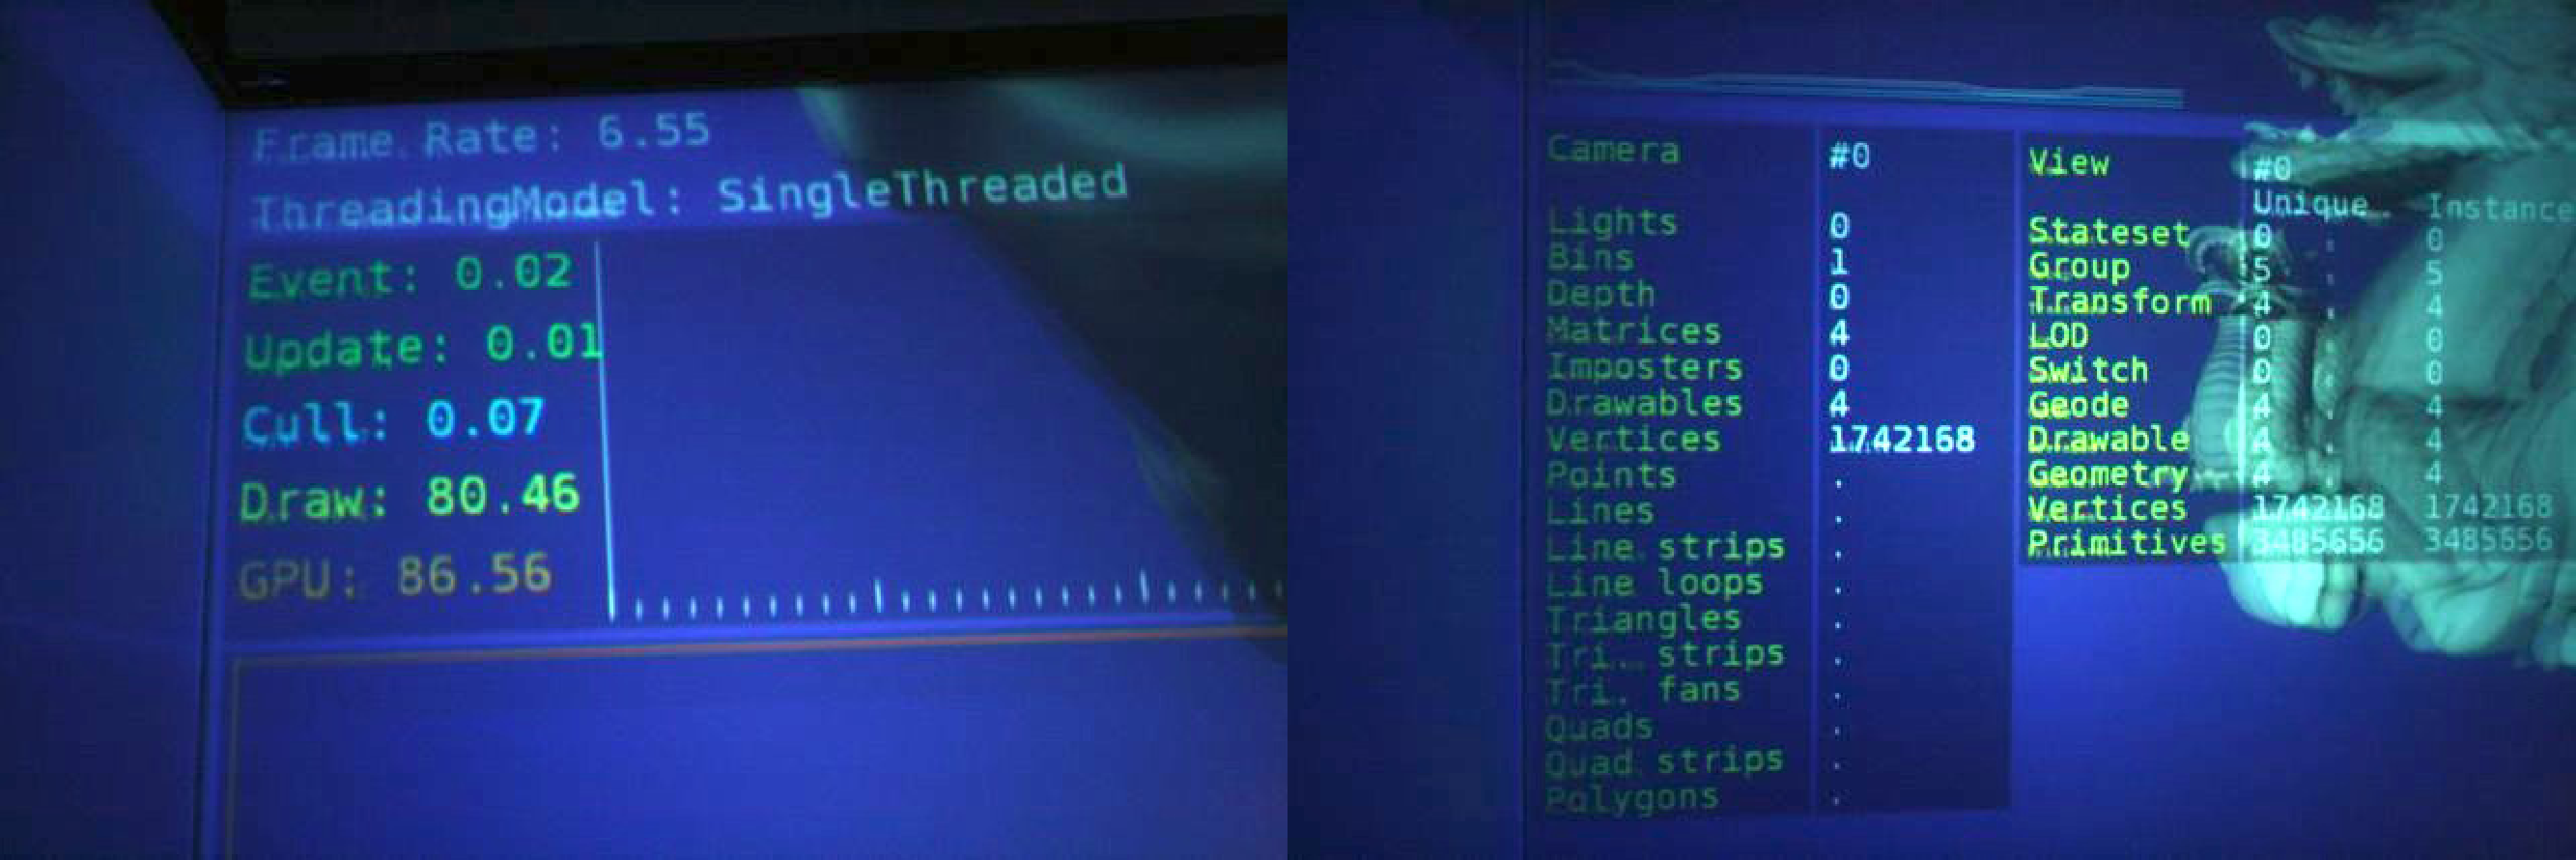
\includegraphics[width=0.9\textwidth]{../figures/fotos/osgStats}
	\caption{OSG statistics}
	\label{fig:osg_stats}
\end{figure}

The most interesting output for our measurements was the \gls{fps}. As mentioned before, we tested two different Equalizer setups. One with a single node, using four graphics cards. The other, a distributed setup with six rendering clients and one server. On the latter, we achieved a more or less constant framerate of 100 \gls{fps} with a model of 1'100'000 triangles. This was about what we expected.

The hardware and software setup as well as the detailed results of the tests can be found in the Technical Report.

Figure \ref{fig:eq_stats} shows the output of Equalizer measured with the multi-node setup. Equalizer orients itself on the slowest rendering client. The green at the bottom of the statistics represents client number six of the setup. It is the slowest client, meaning, it needs the most time to render a single frame. The five other clients listed above need about 1/5 of the time to render a frame.

\begin{figure}[H]
	\centering
	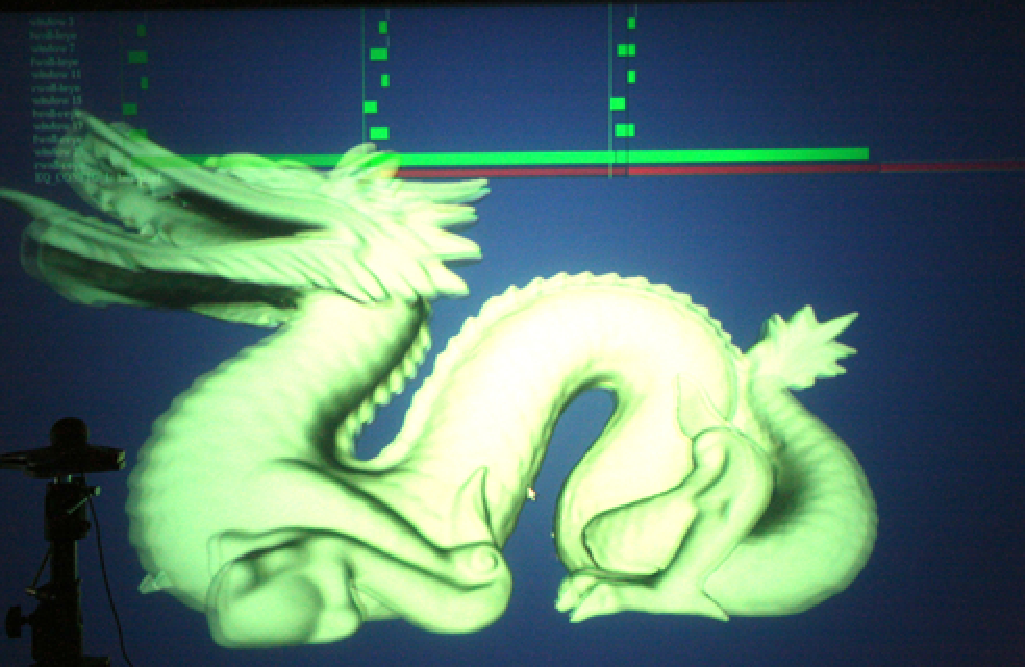
\includegraphics[width=0.5\textwidth]{../figures/fotos/eqStats}
	\caption{Equalizer statistics}
	\label{fig:eq_stats}
\end{figure}
	
The second approach with one computer was less satisfying. With this setup we reached a maximum of 20 \gls{fps}. Conspiciously, the frame rate decreases linearly with each model, even though, they appear on separate walls and should therefore be rendered in different pipes. This behaviour leads to the conclusion that the entire scene graph is rendered on each graphics card. Concerning this issue, we wrote on the Equalizer mailing list. Stefan Eilemann, the founder and developer of Equalizer pointed out that this might be a problem of the NVIDIA graphics driver which could be solved with a later driver release. Other possible reasons he pointed out were:

\begin{itemize}
	\item CPU/Memory contention
	\item Serialisation of the draw calls
	\item Bad multi-threading driver support
	\item Lock contention in \gls{osg} render traversal.
\end{itemize}

The last reason seemed unlikely since the \gls{osg} community never reported similar problems.

\section{Equalizer Conclusion}

Equalizer follows a new approach in parallel rendering. Other than Chromium, it renders the code in parallel and does not send the output over the network. Therefore, it solves the network traffic problem of Chromium.

But this leads to the disadvantage of Equalizer since it requires that an application has to be installed on \emph{all} nodes that are used for rendering. We wrote a script that synchronised our clients after a new release of the application. Otherwise it is very time consuming to update all clients one by one.

Other than that, we could verify the performance results of Equalizer provided by its developers.
